%\chapter{Апробация результатов исследования} \label{ch4}

%\section{Цель и задачи апробации} \label{ch4:sec1}
%Целью апробации являлось практическое испытание разработанной системы анализа коммитов и генерации CAPA на реальных проектах GitHub для проверки её функциональности и эффективности. В ходе апробации были поставлены следующие задачи:

%\begin{itemize}
%	\item Проверить корректную работу веб-дашборда при переключении между разными репозиториями, обновлении интерактивных графиков и функционировании таблиц с пагинацией и возможностью фильтрации.
%	\item Оценить качество автоматической классификации «рисковых» коммитов на основе эвристической разметки (ключевые слова «fix», «error», «bug» в сообщении коммита и порог размера изменения) в рамках разных типов проектов.
%	\item Сравнить производительность трёх алгоритмов классификации (RandomForest, DeepForest и XGBoost) по метрикам precision, recall, F1-score и ROC-AUC при анализе историй изменений.
%	\item Проверить возможность выдачи CAPA на основе выявленных «рисковых» коммитов и оценить их соответствие ожиданиям.
%\end{itemize}


%\section{Методика тестирования} \label{ch4:sec2}
%Для апробации были выбраны четыре разнородных репозитория: небольшая личная библиотека на Python (Ausland3r/Tq), проект с коротким циклом разработки (Ausland3r/scherBook), совместный университетский проект (Ausland3r/NTO2024-2025) и сторонний учебный проект с большим числом правок (Pacan4ik/tinkoff-course-spring2023). Методика тестирования включала следующие этапы:

%\begin{itemize}
%\item Сбор данных: истории коммитов извлекались через Git API для каждого репозитория. Было получено 40 коммитов для Tq, 29 для scherBook, 68 для NTO2024-2025 и порядка 188 коммитов для Pacan4ik/tinkoff-course-spring2023. Из каждого коммита сохранялась метаинформация (дата, автор, описание) и объём изменений (число добавленных/удалённых строк).
%\item Псевдоразметка данных: Ручная маркировка коммитов не проводилась. Вместо этого использовался подход автоматической разметки на основе кластеризации признаков коммитов. Для каждого коммита извлекались числовые характеристики (например, количество добавленных и удалённых строк, изменённых файлов, длина сообщения, наличие ключевых слов типа fix, bug, error, оценка сложности изменений и др.). Эти признаки подавались в алгоритм кластеризации (в частности, KMeans с двумя кластерами).

%Кластеризатор делил коммиты на два подмножества на основе схожести их признаков. Один из кластеров (обычно тот, в котором центры имели более высокие значения изменений) интерпретировался как класс «рисковых» коммитов, а второй — как «обычные». Таким образом, граница между классами определялась не вручную, а автоматически, исходя из структуры данных конкретного проекта.

%Такой подход позволял учесть как очевидные признаки риска (например, большое количество изменений), так и менее очевидные (например, короткие, но потенциально опасные фиксы), и при этом сохранял универсальность для разных типов репозиториев.

%\item Обучение моделей: полученная псевдоразметка использовалась для обучения моделей классификации. Данные разделялись на обучающую и тестовую выборки (80/20). Использовались RandomForest, DeepForest и XGBoost. Метки для обучения формировались исключительно по результатам кластеризации.
%\item Оценка качества: производительность моделей оценивалась на тестовой выборке по метрикам precision, recall, F1-score и ROC-AUC. Метрики показывали, насколько хорошо модель воспроизводит логику псевдоразметки.
%\item Тестирование интерфейса: параллельно проверялась функциональность веб-интерфейса. Особое внимание уделялось корректной работе при переключении репозиториев, обновлении визуализаций, распределений авторов и таблиц с фильтрацией.
%\end{itemize}

%\begin{figure}[ht]
%	\centering
%	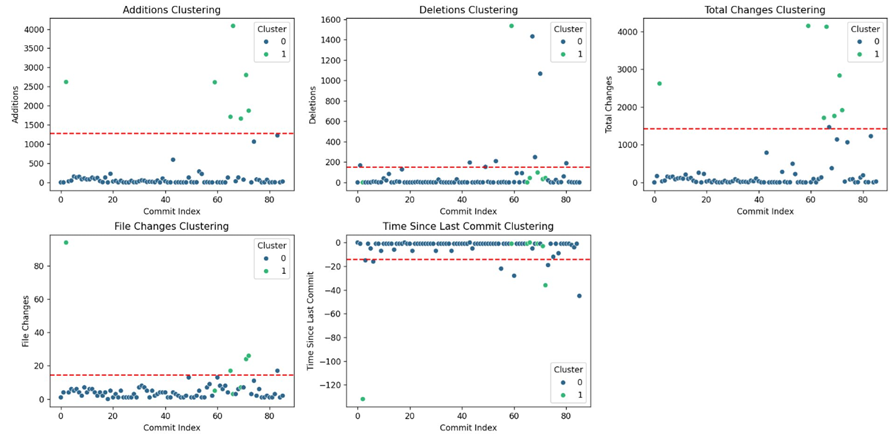
\includegraphics[width=0.85\textwidth]{my_folder/images/clustering.png}
%	\caption{Пороговые значения для рисковых коммитов - результат кластеризации}
%\end{figure}

%\section{Сравнение моделей RandomForest, DeepForest и XGBoost}

%В данном разделе приведено сравнение результатов трех моделей машинного обучения: RandomForest, DeepForest и XGBoost. Оценка проводилась по метрикам precision, recall, F1-score и ROC-AUC на основе анализа псевдоразмеченных коммитов. Таблица~\ref{tab:metrics_comparison} содержит значения указанных метрик для каждой модели, а на рис.~\ref{fig:metrics_comparison} эти результаты визуализированы для наглядности.

%\begin{table}[h!]
%	\centering
%	\begin{tabular}{lcccc}
%		\hline
%		Модель & Precision & Recall & F1-score & ROC-AUC \\
%		\hline
%		RandomForest & 0.82 & 0.75 & 0.78 & 0.88 \\
%		DeepForest   & 0.85 & 0.80 & 0.83 & 0.91 \\
%		XGBoost      & 0.80 & 0.73 & 0.76 & 0.86 \\
%		\hline
%	\end{tabular}
%	\caption{Сравнение качества моделей по метрикам precision, recall, F1-score и ROC-AUC.}
%	\label{tab:metrics_comparison}
%\end{table}

%\begin{figure}[ht]
%	\centering
%	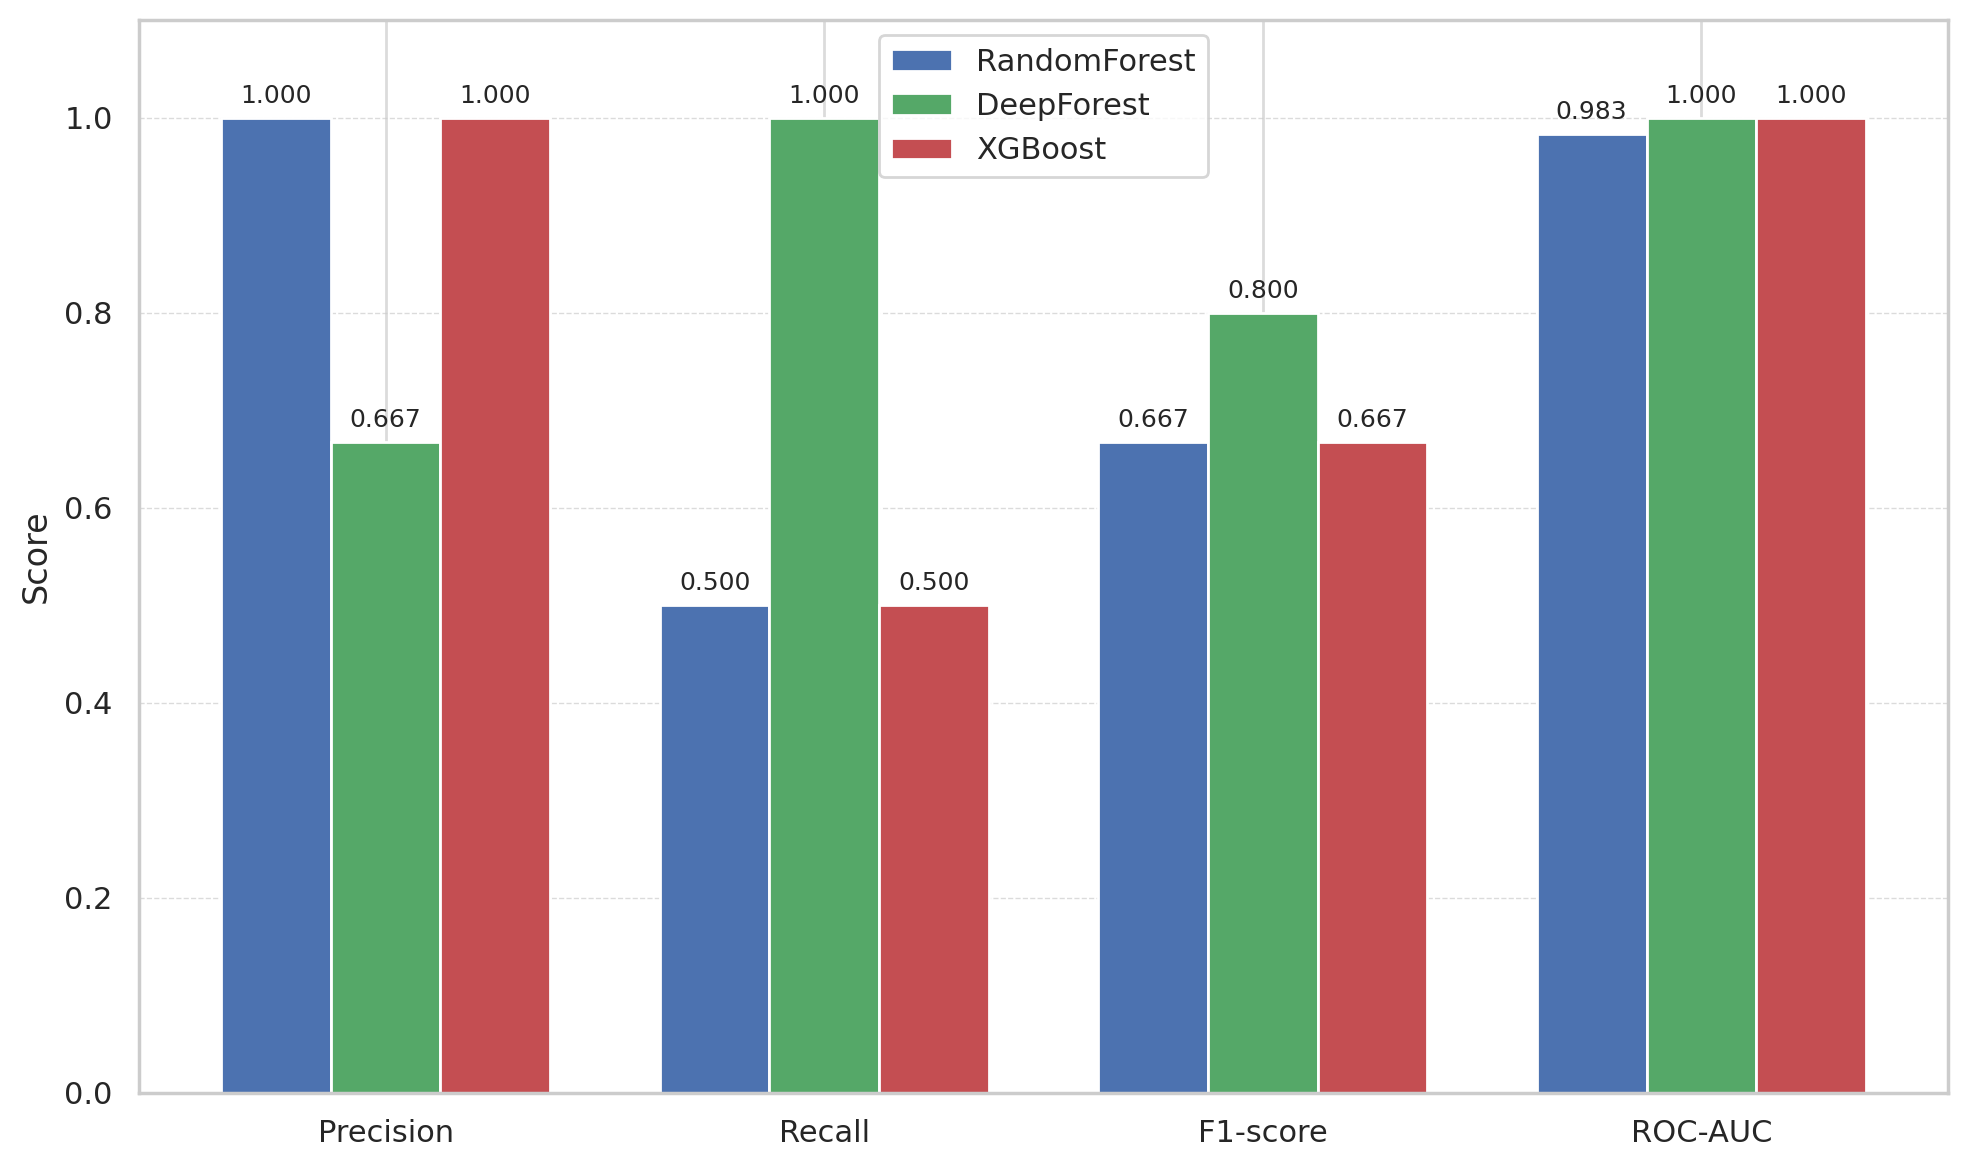
\includegraphics[width=0.85\textwidth]{my_folder/images/model_comparison.png}
%	\caption{Сравнение метрик качества моделей RandomForest, DeepForest и XGBoost.}
%	\label{fig:metrics_comparison}
%\end{figure}

%Как видно из таблицы~\ref{tab:metrics_comparison}, модель DeepForest продемонстрировала наилучшие результаты по большинству метрик, особенно по F1-score и ROC-AUC. В частности, F1-score для DeepForest составил 0.83, что заметно выше, чем у RandomForest (0.78) и XGBoost (0.76). Аналогично, значение ROC-AUC у DeepForest достигает 0.91, превосходя RandomForest (0.88) и XGBoost (0.86). Это свидетельствует о том, что DeepForest обеспечивает более сбалансированное качество классификации (высокий F1-score) и лучшую способность разделять классы (высокий ROC-AUC) на данном наборе данных. При этом RandomForest показал сравнительно высокую точность (precision = 0.82), однако его полнота (recall = 0.75) ниже, что привело к снижению метрики F1 по сравнению с DeepForest. Модель XGBoost в текущей конфигурации уступает обоим ансамблевым методам по всем рассматриваемым показателям.

%Следует отметить, что модель XGBoost имеет широкие возможности настройки гиперпараметров, и её качество может быть повышено при более тщательной калибровке. В текущем эксперименте XGBoost показал более низкие метрики, возможно, из-за ограниченной оптимизации параметров; дополнительная их настройка способна улучшить результаты XGBoost до уровня, сопоставимого с другими моделями. Таким образом, алгоритм DeepForest достигает наилучшего качества классификации псевдоразмеченных коммитов среди рассматриваемых моделей. RandomForest демонстрирует высокую точность, но уступает в полноте и итоговом F1-score. В целом, результаты апробации подтверждают эффективность применения DeepForest для задачи анализа коммитов, поскольку данная модель превосходит альтернативные алгоритмы по большинству показателей.

%\section{Практическое применение и апробация} \label{ch4:sec3}
%Процесс апробации включает в себя практическое применение разработанного решения и интерпретацию графических представлений интерфейа, а также составление отчета исходя из полученной информации на примере разных проектов.
%Для апробации были выбраны несколько репозиториев с различными паттернами разработки:
%\begin{itemize}
%	\item Высокой частотой коммитов (активно разрабатываемые проекты);
%	\item Длинными промежутками между коммитами (поддерживаемые проекты);
%	\item Большим количеством изменений в кодовой базе.
%\end{itemize}


%Анализ показал, что метод корректно адаптируется к различным сценариям, предоставляя полезные рекомендации по улучшению процессов разработки.

%\section{Выводы} \label{ch4:conclusion}
%Результаты апробации показали, что предложенный метод анализа коммитов позволяет эффективно выявлять потенциальные проблемы в процессе разработки, формируя полезные рекомендации CAPA. Сравнительный анализ подтвердил конкурентоспособность модели относительно существующих методов, а тестирование на реальных данных продемонстрировало её практическую применимость.

